\label{sec:results}

\textit{Training was conducted on a Google Colab T4 GPU. Session time limits 
constrained fine-tuning to 3 epochs. The configured maximum was 200. Results below reflect 
this constrained run.}

The model was trained for 3 epochs. Batch size: 128. Optimizer: 
SGD with Nesterov momentum. Scheduler: cosine annealing with linear warm-up, as described in Section~IV. 
Final performance metrics are summarized in Table~\ref{tab:results}.

\begin{table}[h]
\caption{Training and Evaluation Results}
\label{tab:results}
\centering
\begin{tabular}{lcc}
\toprule
\textbf{Split} & \textbf{Loss} & \textbf{Accuracy (\%)} \\
\midrule
Train (epoch 3) & 0.0474 & 99.03 \\
Validation      & 0.0099 & 99.86 \\
Test            & 0.0096 & 99.80 \\
\bottomrule
\end{tabular}
\end{table}

Test accuracy reached \textbf{99.80\%} at epoch 3. Validation accuracy at epoch 1 was 64.41\%. By epoch 3 it reached 99.86\%. Training was 
terminated well short of the configured limit.

These numbers require qualification. The ImageNet-pretrained backbone carries a strong prior. 
The dataset is constrained: controlled backgrounds, consistent framing, one hand per image. High accuracy under these conditions is not a claim of general robustness.

W\&B logs at the final epoch show a mean gradient norm of 1.64 and a clipping ratio of 0.77. The clipping constraint was still active and the loss had not yet flattened. Training to full convergence would likely yield marginal gains on this dataset; the benefit would be more meaningful on harder, 
out-of-distribution evaluation sets.

\begin{figure*}[!t]
    \centering
    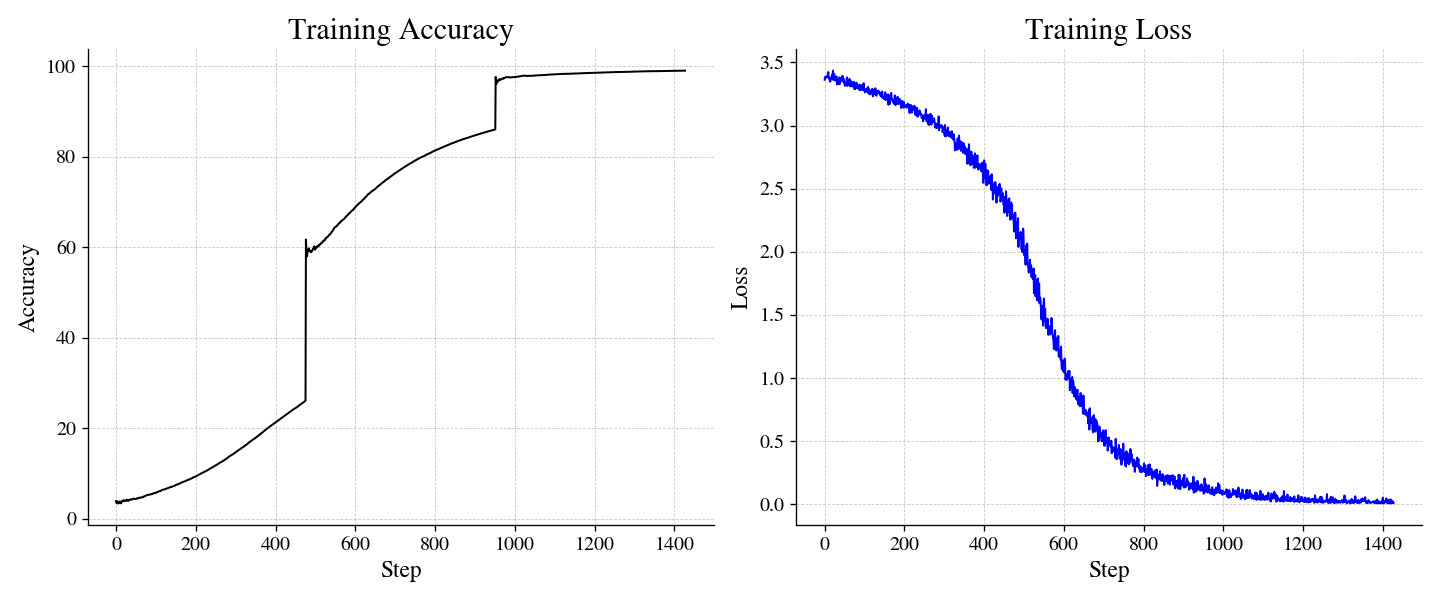
\includegraphics[width=\textwidth]{Training Plots}
    \caption{Training and validation loss/accuracy curves across steps along with gradient norm, 
    logged via Weights \& Biases.}
    \label{fig:training}
\end{figure*}

The main challenge for deployment is distribution shift. 
The training set does not cover varied skin tones, uncontrolled lighting, or cluttered backgrounds. 
The two-stage design helps partially -- MediaPipe isolates the hand crop before it reaches the classifier, 
which cuts down on background interference.

\subsection{Colab Cell Output}
The Colab cell output is attached for reference. 
The full implementation is available at the official GitHub repository: \href{https://github.com/madhavasthana-oss/SLD_MAHE}{github.com/madhavasthana-oss/SLD\_MAHE}.
